\documentclass[fleqn, a4paper. 12pt]{ltjsarticle} 
% following is the compile command (以下のコマンドでコンパイル可能)
% $ lualatex guidance.tex 
% you need to install texlive to execute the above.(texlive を入れる必要がある.)
\usepackage{amsmath,txfonts}
\usepackage{amssymb}
\usepackage{url}
\usepackage{subcaption}
\usepackage[margin=31mm]{geometry}
\usepackage{graphicx}
\usepackage{listings}


\begin{document}
\begin{titlepage}
      \begin{center}
      {
      \Huge 2023年度\\システムプログラミング実験}
      
      \vspace{4cm}
             {\Huge テクニカルライティング\\
               実験レポート\\}
             \vspace{4cm}
                    {\large 実験日:2024年1月24日(水)\\提出日:2024年1月30日(火)\\}
                    
                    {\large 学修番号:22140003\\氏名:佐倉仙汰郎\\ 共同実験者:稲村玲於奈、今村真沙斗}
    \end{center}  
  \end{titlepage}
  
    \section{はじめに}
    本実験ではUser Datagram Protocol (UDP)\footnote{https://datatracker.ietf.org/doc/html/rfc768 (Accessed 2024/1/29)},
    TransmissionControl Protocol (TCP)\footnote{https://datatracker.ietf.org/doc/html/rfc793 (Accessed 2024/1/29)}を用いた基礎的なネットワークを構築する.
    \section{実験の説明}
    C++でUDPとTCPそれぞれの手法を用いてecho機能を実装する.
    クライアントが入力した文字列がクライアントとサーバー側で確認できるようにする.
    また、送信から受信までの時間(Round Trip Time)を測定する.
    UDPとTCPの違いをわかりやすくするために、長い文字列をランダムで生成して送信する機能も実装する.
    長い文字列を生成するためには、文字列を分割して何度かに分けて送信する必要があり、UDPとTCPの送信速度の違いなどを考察するために適していると考える.
    最後にUDPとTCPの違いなどを実験結果から考察を行う.

    \section{開発環境}
    \begin{itemize}
      \item Central Processing Unit: 11th Gen Intel(R) Core(TM) i7-1165G7\footnote{\url{https://www.intel.co.jp/content/www/jp/ja/products/sku/208921/intel-core-i71165g7-processor-12m-cache-up-to-4-70-ghz-with-ipu/specifications.html}}, 2.80 GHz
      \item 主記憶: Double Data Rate 4 Synchronous Dynamic Random-Access Memory\footnote{\url{https://www.jedec.org/standards-documents/docs/jesd79-4a}}, 1200 MHz, 256 bit
      \item コンパイラ: gcc version 11.4.0\footnote{https://gcc.gnu.org/}
      \item コンパイルコマンド: gcc compiler.c (compiler.c はソースプログラムのファイル名である.)
      \item Operating System: Arch Linux\footnote{\url{https://archlinux.org/}} (カーネルは 5.14.8-arch1-1を使用)
  \end{itemize}


    \section{実験結果}
    \subsection{UDP}
    まずはecho機能を実装した.
    getline()で標準入力を受け取りそのクエリを送信するシンプルなコードである.
    何度も送信するために、while文を使っている.
    図\ref{fig:terminal1}のように、クエリを送信し、サーバーからソケットを受け取ると、RTTが表示される.
    標準入力でENDを受け取ると、クライアントのプログラムは終了する.
    またUDPはコネクションを確立せず、送られてきたものにすぐに処理を行うので、同時に複数のクライアントからクエリを送ってもサーバーは受け取ることができる.\\
    バッファを使用するときには必ず終端文字を入れなければならないので、送信するときには必ず終端文字を入れることに気を付けた.
    今回はバッファのサイズを64で設定した.
    したがって64文字以上のクエリを送信するときには、複数回に分けて送信する必要がある。
    図\ref{fig:udp_rand}は、$2^{10}$個から$2^{24}$個のランダムに生成した文字を送信したものである.
    それぞれの送信受信が終わった時に、RTTを別のcsvファイルに書き込んである.
    その結果とグラフについてTCPとの比較のために後述する.
    パケットロスを確認するために、文字の数をmsgcountとして出力している.
    図\ref{fig:udp_rand}からわかる通り、msgcountが、サーバー側とクライアント側で一致していて、パケットロスがないことが確認できる.
    疑似乱数はメルセンヌツイスター法を使用した.\\


    \begin{figure}[htbp]
      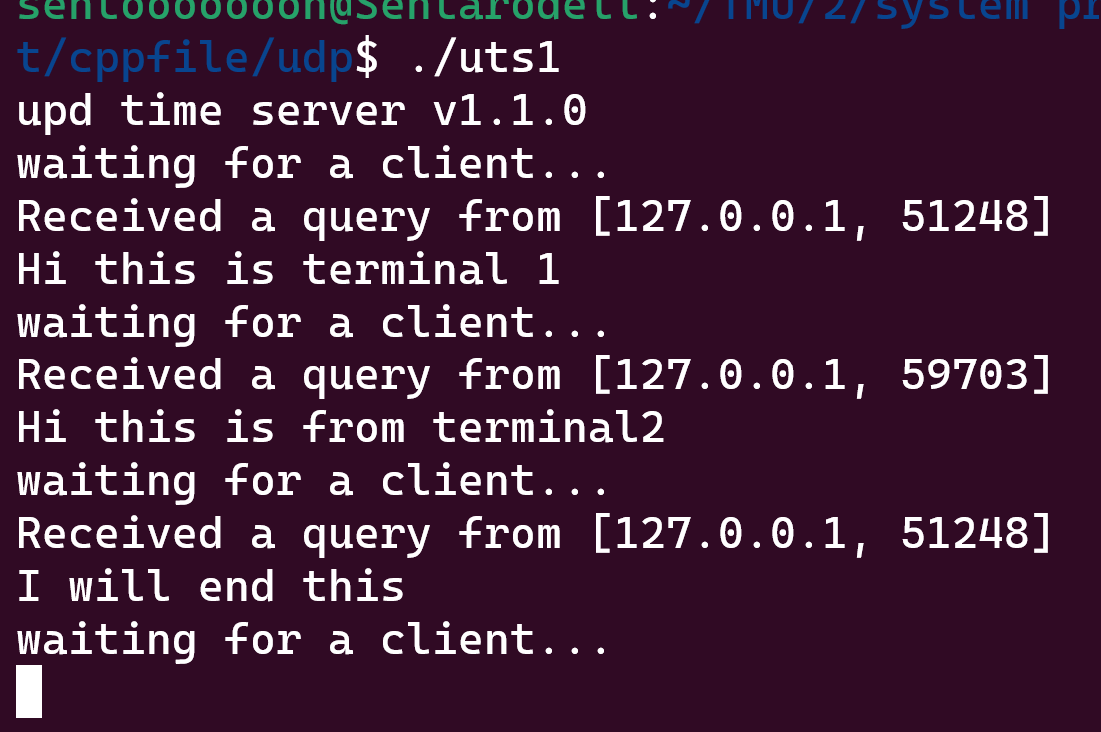
\includegraphics[width=0.5\textwidth]{images/udp_server_echo.png}
      \caption{echo機能のサーバー側}
      \label{fig:udpserver1}
    \end{figure}
    \begin{figure}[htbp]
      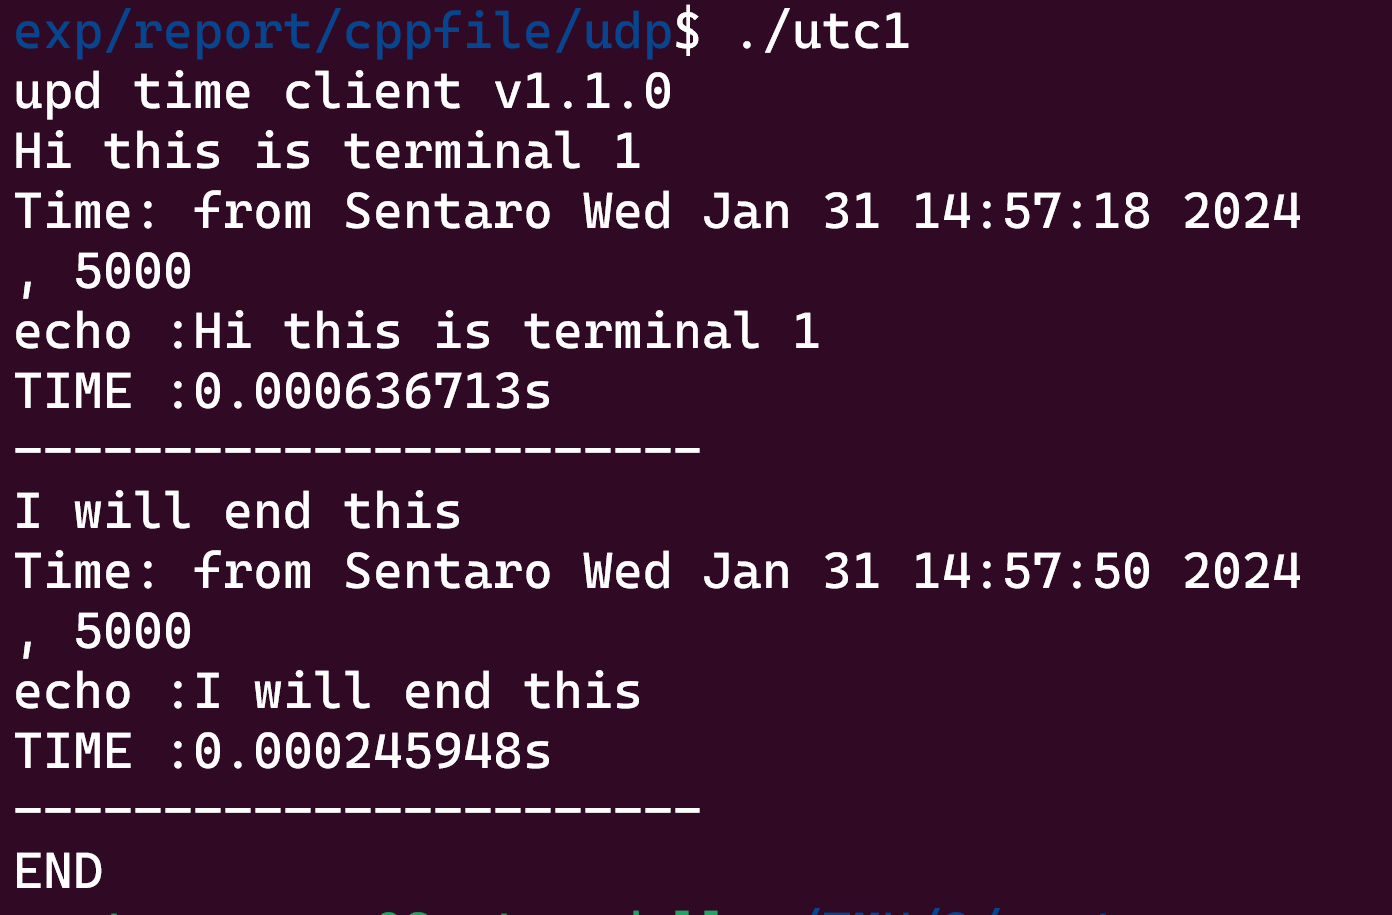
\includegraphics[width=0.5\textwidth]{images/udp_terminal1.png}
      \caption{echo機能のクライアント1}
      \label{fig:terminal1}
    \end{figure}
    \begin{figure}[htbp]
      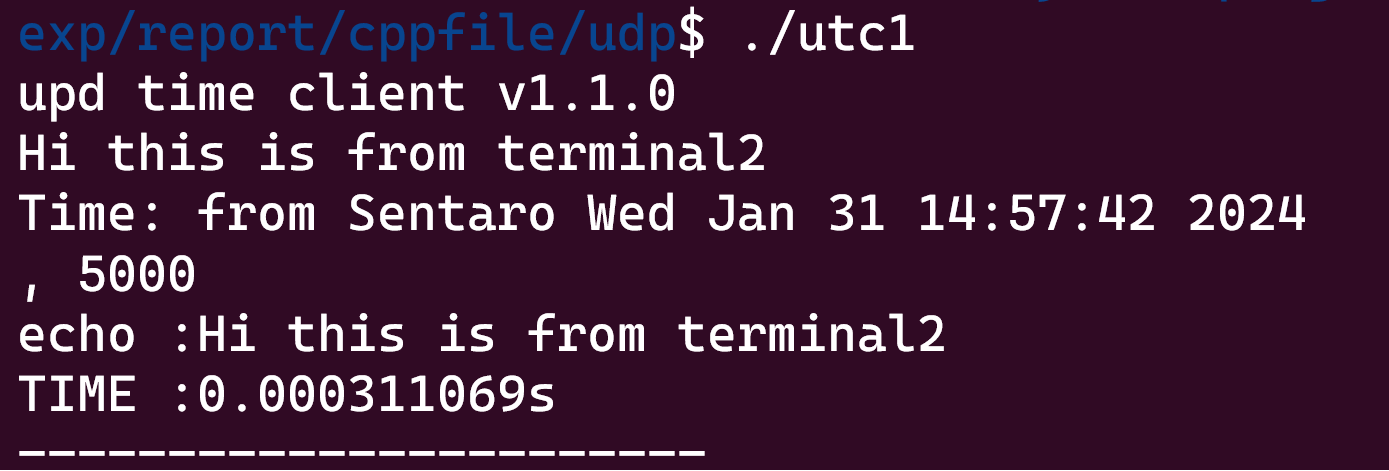
\includegraphics[width=0.5\textwidth]{images/udp_terminal2.png}
      \caption{echo機能のクライアント2}
      \label{fig:terminal2}
    \end{figure}
    
    \begin{figure}[htbp]
      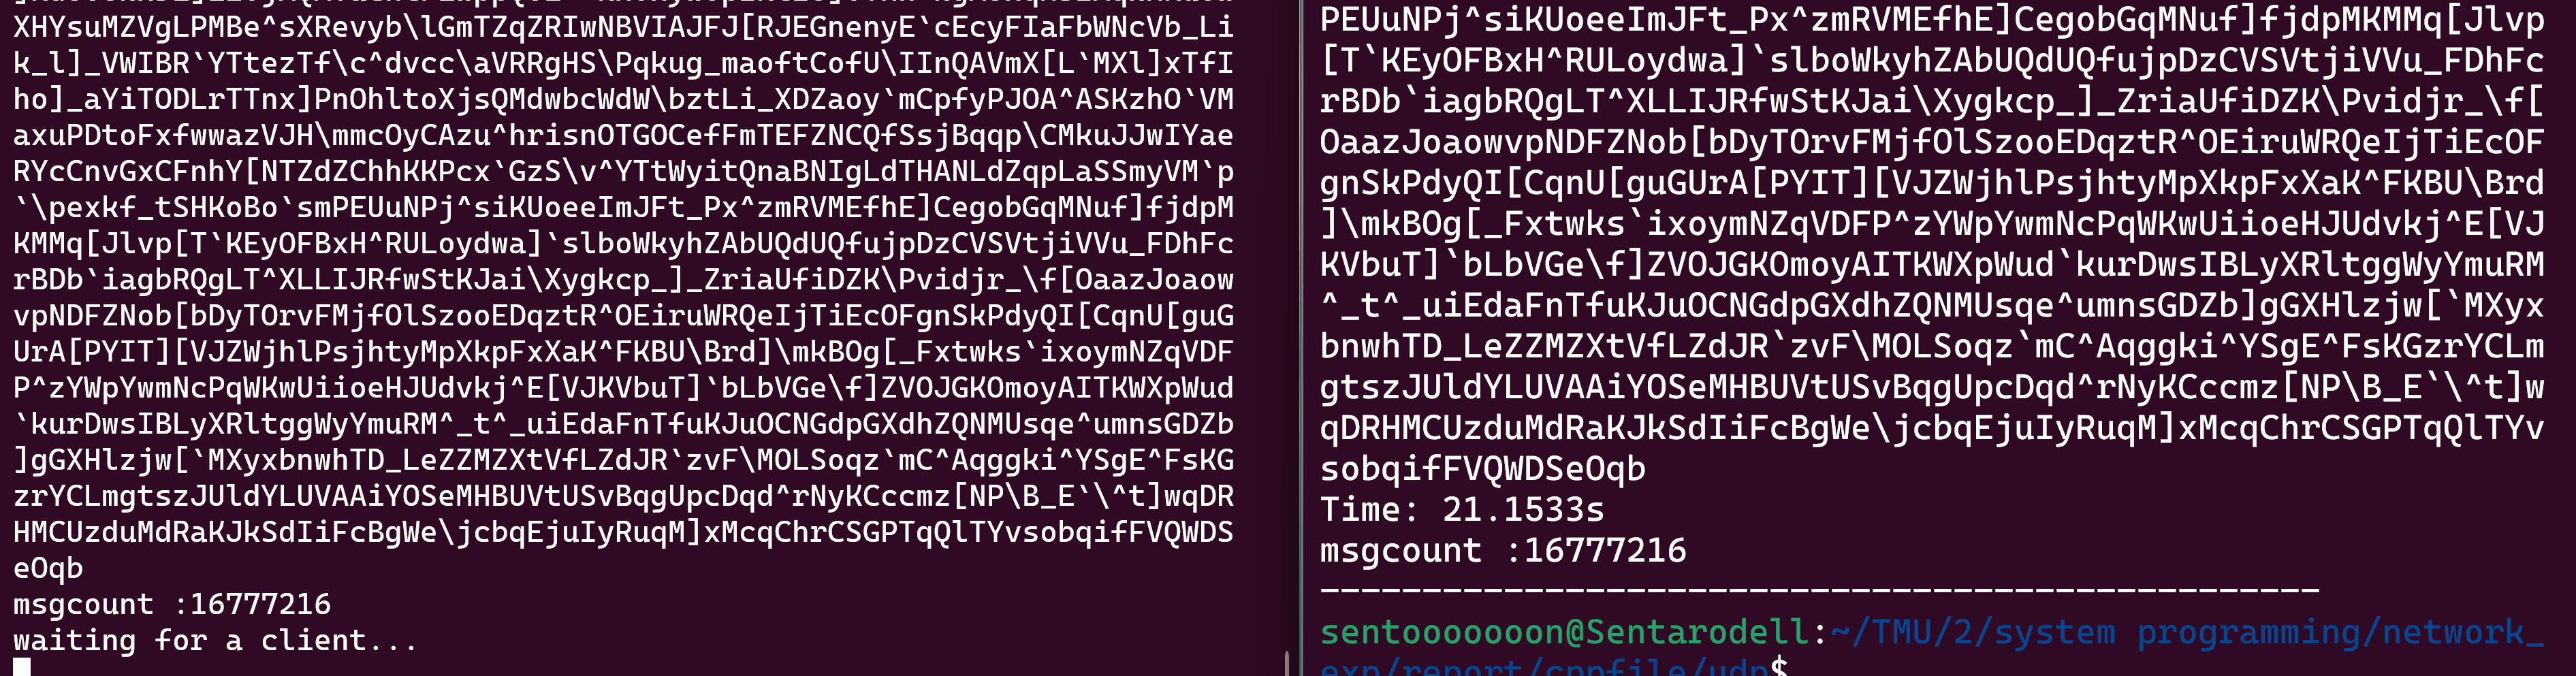
\includegraphics[width=0.5\textwidth]{images/udp_rand.png}
      \caption{ランダムで生成した文字列を送信し、エコーする}
      \label{fig:udp_rand}
    \end{figure}
    
    \newpage
    \subsection{実験結果(TCP)}
    TCPのソースコードも基本的なところはUDPと大きくは変わらない.
    ただ一つ大きな違いとして、TCPはコネクションを確立するため、ループ文のスコープについて気を付けた.
    またコネクションを確立するため、サーバーは一つのクライアントしか対応できない.
    ほかのクライアントがコネクションのためのリクエストを送信しても、接続されているコネクションが切断されるまでは、待機状態となる.
    
    \begin{figure}[htbp]
      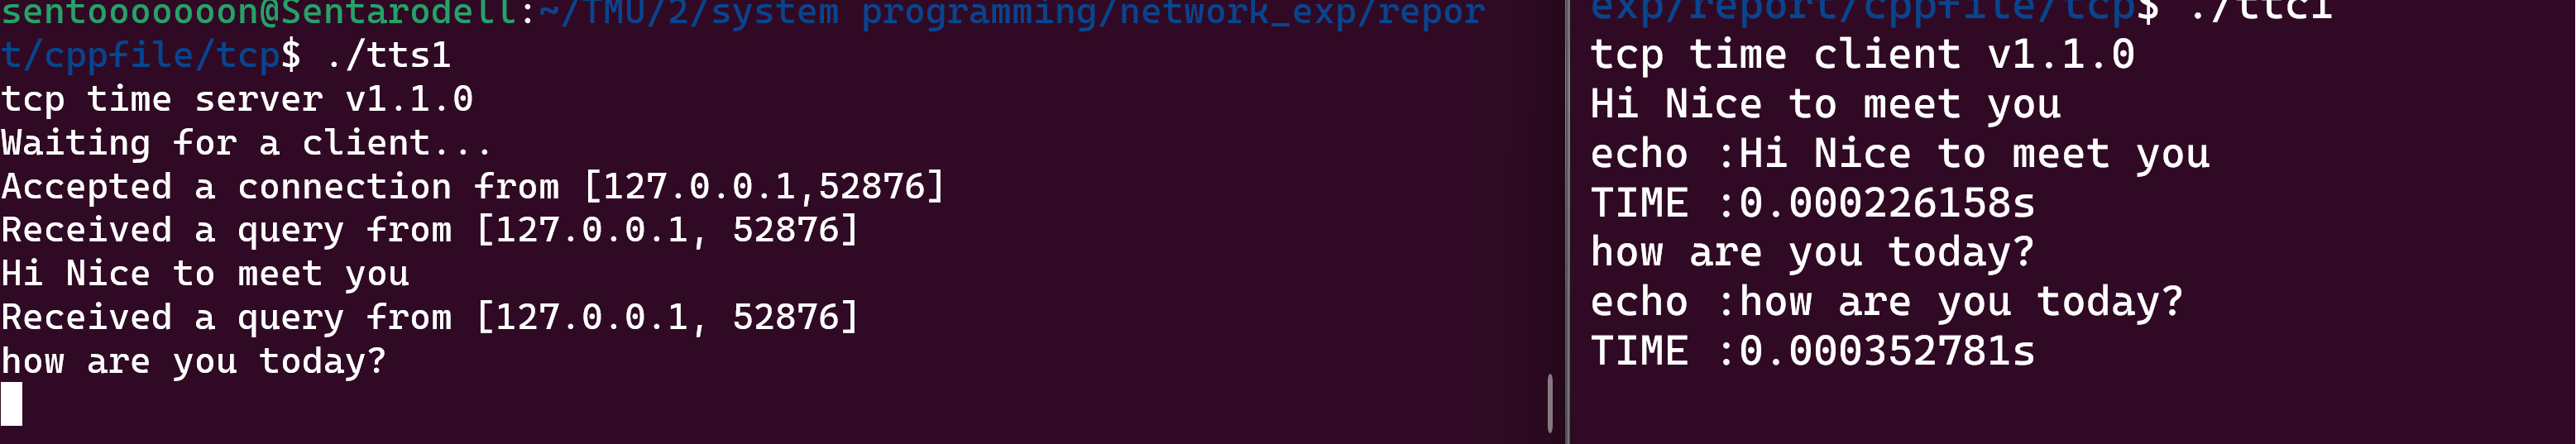
\includegraphics[width=0.5\textwidth]{images/tcp_echo.png}
      \caption{ランダムで生成した文字列を送信し、エコーする}
      \label{fig:udp_rand}
    \end{figure}

    \begin{figure}[htbp]
      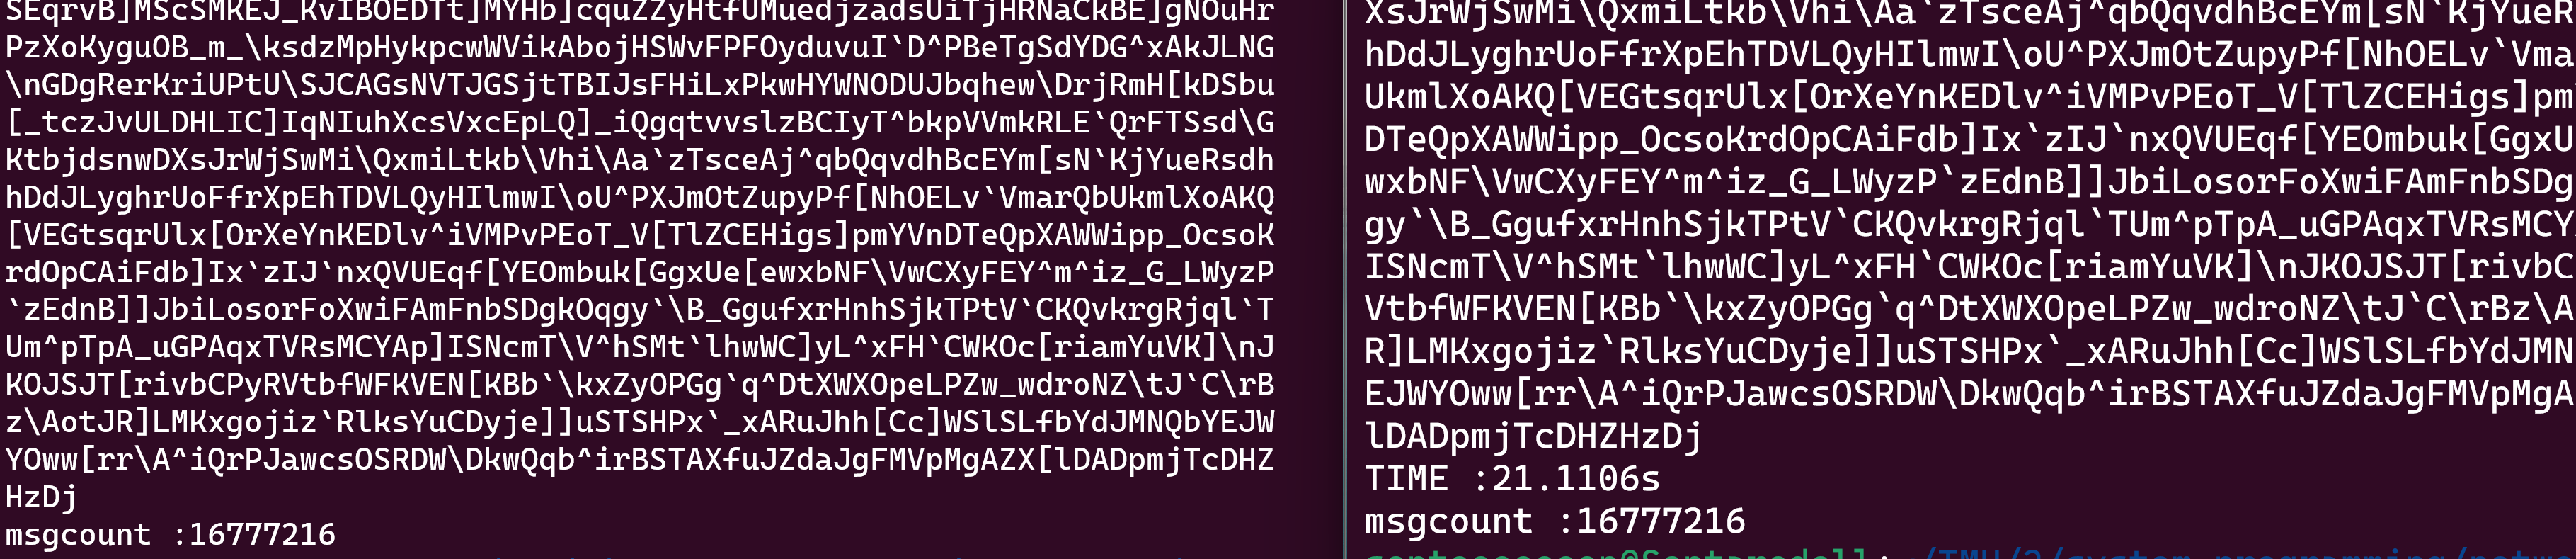
\includegraphics[width=0.5\textwidth]{images/tcp_rand.png}
      \caption{ランダムで生成した文字列を送信し、エコーする}
      \label{fig:udp_rand}
    \end{figure}

    \newpage
    \subsection{UDPとTCPのRTT}

    \begin{figure}[htbp]
      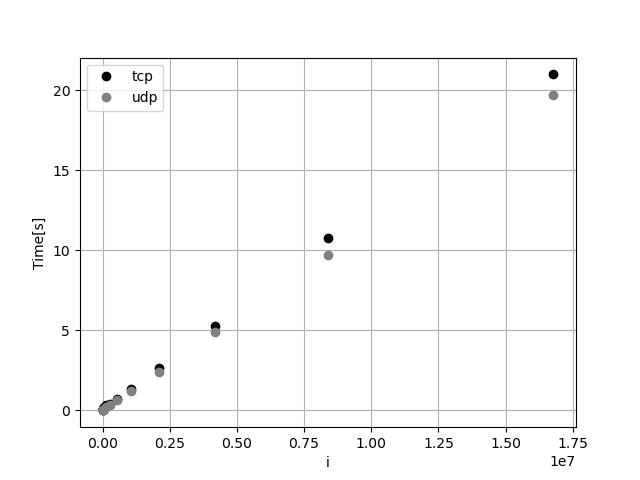
\includegraphics[width=0.5\textwidth]{plot.png}
      \caption{UDPとTCPのRTTのグラフ}
      \label{fig:RTT}
    \end{figure}
    図\ref{fig:RTT}は、$2^{10}から2^{24}$個の文字列をそれぞれの手法を用いて送信したときのRTTである.
    図\ref{fig:RTT}からわかるように、UDPとTCPは文字列の数が増えると処理速度に差がでてくることが分かる.
    今回の実験では、UDPのほうが早いことが分かる.
    一般に、速度はUDPのほうが高いとされていて、今回の実験では、その違いが分かった.
    またUDPは処理速度が速いが、パケットロスの可能性があるとされている.
    今回、パケットロスを確認するために、文字列の数をクライアント側と、サーバー側で数えたが、UDP,TCPでともにすべて一致していた.
    また、この図\ref{fig:RTT}では細かい差が判断できないので、表を用いて結果を示す.
    
  

      \begin{table}[htbp]
        \centering
        \begin{subtable}[b]{0.4\textwidth}
            \centering
            \begin{tabular}{|c|c|c|}
              \cline{1-2}
              i  & Time{[}s{]} &  \\ \cline{1-2}
              10 & 0.003466    &  \\ \cline{1-2}
              11 & 0.004856    &  \\ \cline{1-2}
              12 & 0.011126    &  \\ \cline{1-2}
              13 & 0.016745    &  \\ \cline{1-2}
              14 & 0.033263    &  \\ \cline{1-2}
              15 & 0.066388    &  \\ \cline{1-2}
              16 & 0.086203    &  \\ \cline{1-2}
              17 & 0.169551    &  \\ \cline{1-2}
              18 & 0.322085    &  \\ \cline{1-2}
              19 & 0.634658    &  \\ \cline{1-2}
              20 & 1.27242     &  \\ \cline{1-2}
              21 & 2.64262     &  \\ \cline{1-2}
              22 & 5.24832     &  \\ \cline{1-2}
              23 & 10.2271     &  \\ \cline{1-2}
              24 & 21.1533     &  \\ \cline{1-2}
            \end{tabular}
            \caption{UDP}
            \label{tab:table1}
        \end{subtable}
        \hfill
        \begin{subtable}[b]{0.4\textwidth}
            \centering
            \begin{tabular}{|c|c|c|}
              \cline{1-2}
              i  & time     &  \\ \cline{1-2}
              10 & 0.00128  &  \\ \cline{1-2}
              11 & 0.049361 &  \\ \cline{1-2}
              12 & 0.048579 &  \\ \cline{1-2}
              13 & 0.053925 &  \\ \cline{1-2}
              14 & 0.076731 &  \\ \cline{1-2}
              15 & 0.13745  &  \\ \cline{1-2}
              16 & 0.14284  &  \\ \cline{1-2}
              17 & 0.226125 &  \\ \cline{1-2}
              18 & 0.392836 &  \\ \cline{1-2}
              19 & 0.992046 &  \\ \cline{1-2}
              20 & 1.50903  &  \\ \cline{1-2}
              21 & 2.87307  &  \\ \cline{1-2}
              22 & 5.66146  &  \\ \cline{1-2}
              23 & 11.0475  &  \\ \cline{1-2}
              24 & 21.1106  &  \\ \cline{1-2}
            \end{tabular}
            \caption{TCP}
            \label{tab:table2}
        \end{subtable}
        \caption{RTT of TCP and UDP\\iは$2^{i}$である.}
        \label{tab:tables}
    \end{table}
    表\ref{tab:tables}から、iの値によって差の大小はあるが、TCPのほうが時間がかかる傾向にあることがわかった.

    \section{考察}
    UDPとTCPの処理の差は顕著な差とはならなかった.これは文字列をさらに長くすることで、より差がはっきりすることが予想される.
    図\ref{fig:RTT}から、差が広がる傾向が分かるため、文字列の長さの変更は差をよりはっきりさせるために有効であると考えた.
    また、RTTへ影響を与える可能性があるのは、同時接続台数ではないかと考察する.UDPではいつのサーバーに対し、多数のクライアントからパケットを送ることが可能である.
    パケットの送受信の回数が同じでも、様々な計算器からパケットを送ることで、遅延が生じるのではないかと思った.


    \section{おわりに}
    本実験では、TCPとUDPを用いて、基礎的なネットワークを構築した.
    実験結果より、UDPのほうがTCPより処理が若干高速である.

    \appendix
\section{付録}

\subsection{C++ソースコード}

\begin{lstlisting}[language=C++]


//
// 情報通信応用実験 ネットワークプログラミング
//
// 首都大学東京 システムデザイン学部 情報通信システムコース
// 准教授・酒井和哉
// 2015年2月5日
//
// 情報科学科
// 助教・柴田祐樹
// 2019年10月 改訂
// 2020年10月 改訂
//

#include <arpa/inet.h>
#include <iostream>
#include <chrono>
#include <ctime>
#include <string.h>
#include <unistd.h> // https://linux.die.net/man/2/read

const int BUFF_SIZE = 64; // バッファのサイズ


/*
 * UDP Daytimeクライアント
 */
int main(int argc, char* argv[])
{
    using namespace std;
    using namespace chrono;

    cout << "upd time client v1.1.0" << endl; // ソースコードへの変更を行ったら数値を変える.
    string serv_ip = "127.0.0.1"; // ループバックアドレス
    in_port_t port_num = 5000; // ポート番号
    int n = 0; // 戻り値の保存用
    char buff[BUFF_SIZE]; // 送受信用バッファ

    if (argc == 2) {
        serv_ip = argv[1];
    }
    // パラメータの初期化
    struct sockaddr_in serv_addr; // アドレス構造体
    serv_addr.sin_family = AF_INET;
    serv_addr.sin_addr.s_addr = inet_addr(serv_ip.c_str());
    serv_addr.sin_port = htons(port_num);

    // ソケットの作成.UDPを用いるため第2引数にDatagram,第3引数にUDPを指定する.
    int socketd = socket(AF_INET, SOCK_DGRAM, IPPROTO_UDP);
    if (socketd < 0) {
        cout << "Failed to create a client socket.\n";
        return -1;
    }

    while(1){
    // クエリ送信.('query'という文字列)を送信するだけ.
        string msg;
        getline(cin, msg);
        //cin >> msg;
        //ENDと入力されたら終了.
        if(msg == "END"){
            break;
        }
        auto start = system_clock::now();
        n = sendto(socketd, msg.c_str(), msg.size(), 0, (struct sockaddr*)&serv_addr, sizeof(serv_addr));
        if (n < 0) {
            cout << "failed to receive a message.\n";
            return -1;
        }
        // サーバから現在時刻を文字列として受信.
        n = recvfrom(socketd, buff, sizeof(buff)-1, 0, NULL, NULL); // 終端文字列を入れるために,sizeof(buff)-1 として,文字列一つ分必ず余裕を持たせてデータを受信する.buff をこのまま文字列として使わない場合は全記憶を受信に使う.
        if (n < 0) {
            cout << "Failed to receive a message.\n";
            return -1;
        }
        

        buff[n] = 0; // 終端文字列を追加.送信者が終端文字列を入れてデータを送ってきているとは限らない.
        cout << "Time: " << buff <<", " << htons(serv_addr.sin_port)<< "\n";
        memset(buff, 0, sizeof(buff));

        //echo
        n = recvfrom(socketd, buff, sizeof(buff)-1, 0, NULL, NULL);
        if (n < 0) {
            cout << "Failed to receive a message.\n";
            return -1;
        }

        buff[n] = 0;
        cout << "echo :" << buff << endl;


        auto end = system_clock::now();
        duration<double> elapsed_seconds = end - start;
        cout << "TIME :" << elapsed_seconds.count() << "s" << endl;
        memset(buff, 0, sizeof(buff));
        cout << "-----------------------" << endl;
    }
    // ソケットを閉じる
    close(socketd);
}
\end{lstlisting}

\begin{lstlisting}[language=C++]
  //
  // 情報通信応用実験 ネットワークプログラミング
  //
  // 首都大学東京 システムデザイン学部 情報通信システムコース
  // 准教授・酒井和哉
  // 2015年2月5日
  //
  // 情報科学科
  // 助教・柴田祐樹
  // 2019年10月 改訂
  // 2020年10月 改訂
  //
  
  #include <arpa/inet.h>
  #include <iostream>
  #include <chrono>
  #include <ctime>
  #include <string.h>
  #include <unistd.h> // https://linux.die.net/man/2/read
  
  const int BUFF_SIZE = 64; // バッファのサイズ
  
  /*
   * UDP Daytimeサーバ.
   *
   */
  int main(int argc, char* argv[])
  {
      using namespace std;
      cout << "upd time server v1.1.0" << endl; // ソースコードへの変更を行ったら数値を変える.
  
      // パラメータ
      int port_num = 5000; // 待ち受けポート番号
      struct sockaddr_in serv_addr, clnt_addr; // サーバとクライアントのソケットアドレス
      int serv_socket; // ソケット記述子
      socklen_t addr_len; // アドレス長
      int n = 0; // 戻り値の保存用
  
      char buff[BUFF_SIZE]; // 送信用バッファ
      time_t now; // 現在時刻の保存用変数
  
      // パラーメータ初期化
      serv_addr.sin_family = AF_INET; // IPv4 プロトコルファミリー
      serv_addr.sin_addr.s_addr = INADDR_ANY; // インターネットアドレス
      serv_addr.sin_port = htons(port_num); // ポート番号設定
  
      // ソケット作成
      // 引数にIPv4, データグラム,UDPを指定する.
      serv_socket = socket(AF_INET, SOCK_DGRAM, IPPROTO_UDP);
      if (serv_socket < 0){
          cout << "Fail to create a socket.\n";
      }
      // バインド(ソケットとポートの結合)
      if (bind(serv_socket, (struct sockaddr*)&serv_addr, sizeof(serv_addr)) < 0) {
          cout << "Failed to bind a socket.\n";
          return -1;
      }
  
      // クライアントからのクエリを待ち受け.
      while (true) {
          // クライアントからクエリ文字列を待ち受ける.
          // UDPはコネクションを確立しないため,クライアントがクエリ文字列を送ってくるのを待機.
          cout << "waiting for a client...\n";
          addr_len = sizeof(clnt_addr);
          n = recvfrom(serv_socket, buff, BUFF_SIZE, 0, (struct sockaddr*)&clnt_addr, &addr_len);
          if (n < 0) {
              cout << "failed to read a query from the socket.\n";
              return -1;
          }
  
          cout << "Received a query from [" << inet_ntoa(clnt_addr.sin_addr) << ", " << htons(clnt_addr.sin_port) << "]" << endl;
          cout << buff << endl;
          
          // 現在時刻取得
          time(&now);
          string msg = string("from Sentaro ") + ctime(&now); // string クラスは加算演算子で文字列を結合可能.
  
          // 現在時刻を文字列として,クライアントに送信する.
          n = sendto(serv_socket, msg.c_str(), msg.size(), 0, (struct sockaddr*)&clnt_addr, sizeof(clnt_addr));
          if (n < 0) {
              cout << "Failed to write a message to the socket.\n";
              return -1;
          }
          n = sendto(serv_socket, buff, sizeof(buff) - 1, 0, (struct sockaddr*)&clnt_addr, sizeof(clnt_addr));
          if (n < 0) {
              cout << "Failed to write a message to the socket.\n";
              return -1;
          }
          memset(buff, 0, sizeof(buff));
      }
  
      // ソケットを閉じる.
      close(serv_socket);
      return 0;
  }
  
\end{lstlisting}

\begin{lstlisting}[language=C++]
  //
  // 情報通信応用実験 ネットワークプログラミング
  //
  // 首都大学東京 システムデザイン学部 情報通信システムコース
  // 准教授・酒井和哉
  // 2015年2月5日
  //
  // 情報科学科
  // 助教・柴田祐樹
  // 2019年10月 改訂
  // 2020年10月 改訂
  //
  #include<string.h>
  #include <arpa/inet.h>
  #include <iostream>
  #include <chrono>
  #include <ctime>
  #include<random>
  #include<cmath>
  #include <fstream>
  #include <unistd.h> // https://linux.die.net/man/2/read
  const int BUFF_SIZE = 64; // バッファのサイズ
  
  
  /*
   * UDP Daytimeクライアント
   */
  int main(int argc, char* argv[])
  {
      using namespace std;
      using namespace chrono;
      cout << "upd time client v1.1.0" << endl; // ソースコードへの変更を行ったら数値を変える.
      string serv_ip = "127.0.0.1"; // ループバックアドレス
      in_port_t port_num = 5000; // ポート番号
      int n = 0; // 戻り値の保存用
      char buff[BUFF_SIZE]; // 送受信用バッファ
      //
      
  
      if (argc == 2) {
          serv_ip = argv[1];
      }
      // パラメータの初期化
      struct sockaddr_in serv_addr; // アドレス構造体
      serv_addr.sin_family = AF_INET;
      serv_addr.sin_addr.s_addr = inet_addr(serv_ip.c_str());
      serv_addr.sin_port = htons(port_num);
  
      // ソケットの作成.UDPを用いるため第2引数にDatagram,第3引数にUDPを指定する.
      int socketd = socket(AF_INET, SOCK_DGRAM, IPPROTO_UDP);
      if (socketd < 0) {
          cout << "Failed to create a client socket.\n";
          return -1;
      }
  
      //make a file
      ofstream of("udp_time.csv");
    
      //set random
      random_device rd;
      mt19937_64 mt(rd());
      uniform_int_distribution<char> cU(65, 122);
      for(int i = 10; i < 25; i++){
          
      int power = pow(2,i);
      int count = 0;
      string  msg;
       //generate random message
      for(int i = 0; i < power; i++){
          char c = cU(mt);
          msg += c;
      }
      //cout << "made random message" << endl;
      //cout << msg << endl;
      //cout << "------------------------------------------------" << endl;
    int c = 0; 
    int j = 0;
      auto start = system_clock::now();
    
       while(true){
         if(j == msg.size()){
           c++;
           buff[c] = 0;
           n = sendto(socketd, buff, sizeof(buff), 0, (struct sockaddr*)&serv_addr, sizeof(serv_addr));
               memset(buff, 0, sizeof(buff));
               n = recvfrom(socketd, buff, sizeof(buff), 0, NULL, NULL);
               cout << buff;
           memset(buff, 0, sizeof(buff));
           //cout << "break" << endl;
           break;
         }
         else if(c == BUFF_SIZE - 1){
           buff[c] = 0;
           n = sendto(socketd, buff, sizeof(buff), 0 , (struct sockaddr*)&serv_addr, sizeof(serv_addr));
               memset(buff,0,sizeof(buff));
               n = recvfrom(socketd, buff, sizeof(buff), 0, NULL, NULL);
               cout << buff;
           c = 0;
           //cout << "sent" << endl;
           //cout << buff << endl;
           memset(buff, 0 ,sizeof(buff));
         }
         //cout << j << endl;
         buff[c] = msg[j]; j++; c++;
       }
       buff[0] = '~';
       buff[1] = 0;
       n = sendto(socketd, buff, sizeof(buff), 0, (struct sockaddr*)&serv_addr, sizeof(serv_addr));
  
      cout <<endl;
  
      //if(msg == "END")break;
      //n = sendto(socketd, buff, BUFF_SIZE, 0, (struct sockaddr*)&serv_addr, sizeof(serv_addr));
      if (n < 0) {
          cout << "failed to receive a message.\n";
          return -1;
      }
      // サーバから現在時刻を文字列として受信.
      //cout << "befor recieve" << endl;
      //n = recvfrom(socketd, buff, sizeof(buff)-1, 0, NULL, NULL); // 終端文字列を入れるために,sizeof(buff)-1 として,文字列一つ分必ず余裕を持たせてデータを受信する.buff をこのまま文字列として使わない場合は全記憶を受信に使う.
      if (n < 0) {
          cout << "Failed to receive a message.\n";
          return -1;
      }
      //cout << "after recieve" << endl;
      auto end = system_clock::now();
  
      duration<double> elapsed_seconds = end - start;
  
      buff[n] = 0; // 終端文字列を追加.送信者が終端文字列を入れてデータを送ってきているとは限らない.
      cout << "Time: " << elapsed_seconds.count() << "s" << "\n";
      memset(buff, 0, sizeof(buff));
      cout << "msgcount :" << msg.size() << endl;
      cout << "-------------------------------------------------" << endl;
      of << i << ","<< elapsed_seconds.count() << endl;
      }
      
    //cout << "end" <<endl;
      // ソケットを閉じる
      close(socketd);
  }
\end{lstlisting}

\begin{lstlisting}[language=C++]
  //
  // 情報通信応用実験 ネットワークプログラミング
  //
  // 首都大学東京 システムデザイン学部 情報通信システムコース
  // 准教授・酒井和哉
  // 2015年2月5日
  //
  // 情報科学科
  // 助教・柴田祐樹
  // 2019年10月 改訂
  // 2020年10月 改訂
  //
  
  #include <arpa/inet.h>
  #include <iostream>
  #include <chrono>
  #include <ctime>
  #include <unistd.h> // https://linux.die.net/man/2/read
  #include<string.h>
  const int BUFF_SIZE = 64; // バッファのサイズ
  
  /*
   * UDP Daytimeサーバ.
   *
   */
  int main(int argc, char* argv[])
  {
      using namespace std;
      cout << "upd time server v1.1.0" << endl; // ソースコードへの変更を行ったら数値を変える.
  
      // パラメータ
      int port_num = 5000; // 待ち受けポート番号
      struct sockaddr_in serv_addr, clnt_addr; // サーバとクライアントのソケットアドレス
      int serv_socket; // ソケット記述子
      socklen_t addr_len; // アドレス長
      int n = 0; // 戻り値の保存用
  
  
      char buff[BUFF_SIZE]; // 送信用バッファ
      time_t now; // 現在時刻の保存用変数
  
      // パラーメータ初期化
      serv_addr.sin_family = AF_INET; // IPv4 プロトコルファミリー
      serv_addr.sin_addr.s_addr = INADDR_ANY; // インターネットアドレス
      serv_addr.sin_port = htons(port_num); // ポート番号設定
  
      // ソケット作成
      // 引数にIPv4, データグラム,UDPを指定する.
      serv_socket = socket(AF_INET, SOCK_DGRAM, IPPROTO_UDP);
      if (serv_socket < 0){
          cout << "Fail to create a socket.\n";
      }
      // バインド(ソケットとポートの結合)
      if (bind(serv_socket, (struct sockaddr*)&serv_addr, sizeof(serv_addr)) < 0) {
          cout << "Failed to bind a socket.\n";
          return -1;
      }
  
      // クライアントからのクエリを待ち受け.
  while (true) {
          // クライアントからクエリ文字列を待ち受ける.
          // UDPはコネクションを確立しないため,クライアントがクエリ文字列を送ってくるのを待機.
          cout << "waiting for a client...\n";
          addr_len = sizeof(clnt_addr);
          int msgcount = 0;
    while(1){
          n = recvfrom(serv_socket, buff, sizeof(buff), 0, (struct sockaddr*)&clnt_addr, &addr_len);
          if (n < 0) {
              cout << "failed to read a query from the socket.\n";
              return -1;
          
    }
    
    if(buff[0] == '~')break;
    //buff[n] = '\0';
    for(int i = 0; i < sizeof(buff); i++){
          if(buff[i]){
              msgcount++;
              cout << buff[i];
          }
    }
      n = sendto(serv_socket, buff, sizeof(buff), 0, (struct sockaddr*)&clnt_addr, sizeof(clnt_addr));
    /*if(sizeof(buff) != BUFF_SIZE){
      break;}
    }*/
  
      //cout << "Received a query from [" << inet_ntoa(clnt_addr.sin_addr) << ", " << htons(clnt_addr.sin_port) << "]" << endl;
      memset(buff, 0, sizeof(buff));
  
  }
    cout << endl;
    // 現在時刻取得
          //time(&now);
          //string msg = string("from shibata ") + ctime(&now); // string クラスは加算演算子で文字列を結合可能.
  
          // 現在時刻を文字列として,クライアントに送信する.
          //n = sendto(serv_socket, msg.c_str(), msg.size(), 0, (struct sockaddr*)&clnt_addr, sizeof(clnt_addr));
          if (n < 0) {
              cout << "Failed to write a message to the socket.\n";
              return -1;
          }
          cout <<"msgcount :" << msgcount << endl;
    //cout << endl;
  }
  
      // ソケットを閉じる.
      close(serv_socket);
      return 0;
  }
\end{lstlisting}

\begin{lstlisting}[language=C++]
  //
  // 情報通信応用実験 ネットワークプログラミング
  //
  // 首都大学東京 システムデザイン学部 情報通信システムコース
  // 准教授・酒井和哉
  // 2015年2月5日
  //
  // 情報科学科
  // 助教・柴田祐樹
  // 2019年10月 改訂
  // 2020年10月 改訂
  //
  
  #include <arpa/inet.h>
  #include <iostream>
  #include <unistd.h> // https://linux.die.net/man/2/read
  #include <string>
  #include <string.h>
  #include <ctime>
  #include <chrono>
  const int BUFF_SIZE = 64; // バッファのサイズ
  
  int main(int argc, char* argv[])
  {
      using namespace std;
      using namespace chrono;
      cout << "tcp time client v1.1.0" << endl; // ソースコードへの変更を行ったら数値を変える.
  
      // サーバのアドレスとポート番号
      // 127.0.0.1は,ループバックアドレス
      // 他のPCと通信する場合は,当該PCのIPアドレスに変更する.
      string serv_ip = "127.0.0.1";
      in_port_t serv_port = 5000;
      
      if(argc > 1)
      {
        serv_ip = argv[1];
      }
      char buff[BUFF_SIZE];// 受信用バッファ
      int n = 0; // 戻り値の保存用に使う変数.
  
      // ソケット作成,入力はIP,ストリーム型,TCPを指定.
      int socketd = socket(AF_INET, SOCK_STREAM, IPPROTO_TCP);
      if (socketd < 0) {
          cout << "Failed to createa socket\n";
          return -1;
      }
      // サーバのアドレス等を初期化.
      struct sockaddr_in serv_addr;
      serv_addr.sin_family = AF_INET;
      serv_addr.sin_addr.s_addr = inet_addr(serv_ip.c_str());
      serv_addr.sin_port = htons(serv_port);
  
      // サーバに接続する.
      n = connect(socketd, (struct sockaddr*)&serv_addr, sizeof(serv_addr));
      if (n < 0) {
          cout << "Failed to connect to the server\n";
          return -1;
      }
      string msg;
              while(true){
              getline(cin, msg);
              auto start = system_clock::now();
              n = write(socketd, msg.c_str(), msg.size()); // 文字列の送信.第二引数は記憶域.第3引数は送信するByte数.
              if(msg == "END"){
                  break;
              }
              // 接続すると,サーバは現在時刻を文字列として返信する.
              // read(.)により,データを受信する.
              n = read(socketd, buff, sizeof(buff)-1);
              if (n < 0) {
                  // readの戻り値が負の場合,通信に不具合が生じたことを意味する.
                  cout << "failed to read from a socket\n";
                  return -1;
              }
              // readの戻り値が 0 の場合,相手が接続を遮断したことを意味する.
              buff[n] = 0;
              // サーバからの返信された文字列(現在時刻)を表示
              /*n = read(socketd, buff, sizeof(buff)-1);
              if (n < 0) {
                  // readの戻り値が負の場合,通信に不具合が生じたことを意味する.
                  cout << "failed to read from a socket\n";
                  return -1;
              }*/
              cout << "echo :";
              for(int i = 0; i < sizeof(buff); i++){
                  cout << buff[i];
              }
              cout <<endl;
              auto end = system_clock::now();
              duration<double> elapsed_seconds = end - start;
              cout << "TIME :" << elapsed_seconds.count() << "s" << endl;
              memset(buff, 0, sizeof(buff));
          }
      // close the socket
      close(socketd);
  }
  
\end{lstlisting}

\begin{lstlisting}[language=C++]
  //
  // 情報通信応用実験 ネットワークプログラミング
  //
  // 首都大学東京 システムデザイン学部 情報通信システムコース
  // 准教授・酒井和哉
  // 2015年2月5日
  //
  // 情報科学科
  // 助教・柴田祐樹
  // 2019年10月 改訂
  // 2020年10月 改訂
  //
  
  #include <arpa/inet.h>
  #include <iostream>
  #include <chrono>
  #include <string.h>
  #include <ctime>
  #include <unistd.h> // https://linux.die.net/man/2/read
  
  const int BUFF_SIZE = 64; // バッファのサイズ
  
  int main(int argc, char *argv[])
  {
      // パラメータ
      using namespace std;
      cout << "tcp time server v1.1.0" << endl; // ソースコードへの変更を行ったら数値を変える.
  
      int port_num = 5000; // ポート番号
  
      struct sockaddr_in serv_addr, clnt_addr; // ソケットアドレス
      int serv_socket, clnt_socket;            // ソケット記述子
      socklen_t addr_len;                      // アドレス長
      int n;                                   // 戻り値の保存用
  
      time_t now;           // 時間
      char buff[BUFF_SIZE]; // 送信用バッファ(64バイト)
  
      // パラメータの初期化
      serv_addr.sin_family = AF_INET;
      serv_addr.sin_addr.s_addr = INADDR_ANY;
      serv_addr.sin_port = htons(port_num);
      addr_len = sizeof(clnt_addr);
  
      // 接続要求受付用のソケットを作成。
      // ソケット記述子(Socket descripter)が戻り値であるが、エラーが起こった場合は「-1」が返される。
      serv_socket = socket(AF_INET, SOCK_STREAM, IPPROTO_TCP);
      if (serv_socket < 0)
      {
          cout << "Failed to create a socket.\n";
          return -1;
      }
      // バインド(ソケットとポートの結合)
      if (bind(serv_socket, (struct sockaddr *)&serv_addr, sizeof(serv_addr)) < 0)
      {
          cout << "Failed to bind a socket to the system.\n";
          return -1;
      }
      // ソケットをコネクション受け入れ可能な状態にする。
      // 第2引数は、接続キューのサイズ。5つまで同時接続を受け入れると指定。
      if (listen(serv_socket, 5) < 0)
      {
          cout << "Filaed to listen to a socket.\n";
          return -1;
      }
  
      // クライアントから接続要求があれば、順次対応
      while (true)
      {
          memset(buff, 0, sizeof(buff));
          // accept(.)により、クライアントからの接続要求を受け付ける。
          // 戻り値はクライアントとのデータ通信用ソケット記述子、エラーの場合は0以下の値が返される。
          cout << "Waiting for a client..." << endl;
          clnt_socket = accept(serv_socket, (struct sockaddr *)&clnt_addr, &addr_len);
  
          // クライアントのIPアドレスとポート番号を表示。
          // それぞれ、struct sockaddr_inから取得。
          // inet_ntoa(.)は、arpa/inet.hで定義されている(Unix系の場合)。 htons はエンディアンを変換する.
          cout << "Accepted a connection from [" << inet_ntoa(clnt_addr.sin_addr) << "," << htons(clnt_addr.sin_port) << "]" << endl;
          while(1){
  
          n = read(clnt_socket, buff, sizeof(buff) - 1);
          cout << "Received a query from [" << inet_ntoa(clnt_addr.sin_addr) << ", " << htons(clnt_addr.sin_port) << "]" << endl;
          if(n <= 0){
              // 相手の通信が切断されている.
              return -1;
          }
          buff[n] = 0; // 文字列として他の関数に渡す場合は,終端文字を追加することを忘れないように気をつける.
          if(buff[0] == 'E' && buff[1] == 'N' && buff[2] == 'D'){
              break;
          }
          cout << buff << endl;
          
          
          // time(.)で現在時間取得(秒単位の歴時間)、ctime(.)で文字列に変換し、送信バッファに書き込み。
          //time(&now);
  
          //string msg = ctime(&now);
  
          // クライアントソケットにバッファの内容を書き込む。
          //n = write(clnt_socket, msg.c_str(), msg.size());
  
  
          n = write(clnt_socket, buff, sizeof(buff)-1);
          
      }
          // クライアントとの通信は終了したので、ソケットを閉じる。
          close(clnt_socket);
      }
      // 受付用のソケットを閉じる。
      close(serv_socket);
      return 0;
  }
  
\end{lstlisting}

\begin{lstlisting}[language=C++]
  //
  // 情報通信応用実験 ネットワークプログラミング
  //
  // 首都大学東京 システムデザイン学部 情報通信システムコース
  // 准教授・酒井和哉
  // 2015年2月5日
  //
  // 情報科学科
  // 助教・柴田祐樹
  // 2019年10月 改訂
  // 2020年10月 改訂
  //
  
  #include <arpa/inet.h>
  #include <iostream>
  #include <unistd.h> // https://linux.die.net/man/2/read
  #include <string>
  #include<string.h>
  #include<chrono>
  #include <ctime>
  #include <cmath>
  #include<random>
  #include <fstream>
  const int BUFF_SIZE = 64; // バッファのサイズ
  
  int main(int argc, char* argv[])
  {
      using namespace std;
      using namespace chrono;
      cout << "tcp time client v1.1.0" << endl; // ソースコードへの変更を行ったら数値を変える.
  
      // サーバのアドレスとポート番号
      // 127.0.0.1は,ループバックアドレス
      // 他のPCと通信する場合は,当該PCのIPアドレスに変更する.
      string serv_ip = "127.0.0.1";
      in_port_t serv_port = 5000;
      
      if(argc > 1)
      {
        serv_ip = argv[1];
      }
      char buff[BUFF_SIZE];// 受信用バッファ
      int n = 0; // 戻り値の保存用に使う変数.
  
      // ソケット作成,入力はIP,ストリーム型,TCPを指定.
      int socketd = socket(AF_INET, SOCK_STREAM, IPPROTO_TCP);
      if (socketd < 0) {
          cout << "Failed to createa socket\n";
          return -1;
      }
      // サーバのアドレス等を初期化.
      struct sockaddr_in serv_addr;
      serv_addr.sin_family = AF_INET;
      serv_addr.sin_addr.s_addr = inet_addr(serv_ip.c_str());
      serv_addr.sin_port = htons(serv_port);
  
      //make a file
      ofstream of("tcp_time.csv");
  
      
      
      // サーバに接続する.
      n = connect(socketd, (struct sockaddr*)&serv_addr, sizeof(serv_addr));
      if (n < 0) {
          cout << "Failed to connect to the server\n";
          return -1;
      }
      //ランダムにメッセージを生成
      
      random_device rd;
      mt19937_64 mt(rd());
      uniform_int_distribution<char> cU(65, 122);
      
      
      //cout << msg << endl;
      //cout <<"----------------------------"<< endl;
  
  
      //string msg = "hello\n";
      for(int i = 10; i < 25; i++){
      
      int power = pow(2,i);
      string msg;
      for(int i = 0; i < power; i++){
          char c = cU(mt);
          msg += c;
        
      }
      int j = 0;
      int c = 0;
  
      auto start = system_clock::now();
      while(true){
         if(j == msg.size()){
           c++;
           buff[c] = '\0';
           n = write(socketd, buff, sizeof(buff));
           memset(buff, 0, sizeof(buff));
               n = read(socketd, buff, sizeof(buff));
              if (n < 0) {
                  // readの戻り値が負の場合,通信に不具合が生じたことを意味する.
                  cout << "failed to read from a socket\n";
                  return -1;
              }
              for(int i = 0; i < sizeof(buff); i++){
                  if(buff[i]){
                      cout <<buff[i];
                  }
              }
           //cout << "break" << endl;
           break;
         }
         else if(c == BUFF_SIZE - 1){
           buff[c] == '\0';
           n = write(socketd, buff, sizeof(buff));
           c = 0;
               n = read(socketd, buff, sizeof(buff));
              if (n < 0) {
                  // readの戻り値が負の場合,通信に不具合が生じたことを意味する.
                  cout << "failed to read from a socket\n";
                  return -1;
              }
              for(int i = 0; i < sizeof(buff); i++){
                  if(buff[i]){
                      cout <<buff[i];
                  }
              }
          //cout << "sent" << endl;
           //cout << buff << endl;
           memset(buff, 0 ,sizeof(buff));
         }
         //cout << j << endl;
         buff[c] = msg[j]; j++; c++;
       }
       //cout << "end loop" << endl;
       buff[0] = '~';
       buff[1] = 0;
  
      n = write(socketd, buff, sizeof(buff)); // 文字列の送信.第二引数は記憶域.第3引数は送信するByte数.
      memset(buff, 0, sizeof(buff));
      // 接続すると,サーバは現在時刻を文字列として返信する.
      // read(.)により,データを受信する.
      
      // readの戻り値が 0 の場合,相手が接続を遮断したことを意味する.
      //buff[n] = 0;
      // サーバからの返信された文字列(現在時刻)を表示
      //cout << buff;
  
      auto end = system_clock::now();
      duration<double> elapsed_seconds = end - start;
      cout << endl;
      cout << "TIME :" << elapsed_seconds.count() << "s" << endl;
      cout << "msgcount :" << msg.size() << endl;
      of << i <<"," << elapsed_seconds.count() << endl;
      //cout << i << endl;
      }
  
      // close the socket
      close(socketd);
  }
  
\end{lstlisting}

\begin{lstlisting}[language=C++]
  //
  // 情報通信応用実験 ネットワークプログラミング
  //
  // 首都大学東京 システムデザイン学部 情報通信システムコース
  // 准教授・酒井和哉
  // 2015年2月5日
  //
  // 情報科学科
  // 助教・柴田祐樹
  // 2019年10月 改訂
  // 2020年10月 改訂
  //
  
  #include <arpa/inet.h>
  #include <iostream>
  #include <chrono>
  #include <ctime>
  #include <string.h>
  #include <unistd.h> // https://linux.die.net/man/2/read
  
  const int BUFF_SIZE = 64; // バッファのサイズ
  
  int main(int argc, char *argv[])
  {
      // パラメータ
      using namespace std;
      
      cout << "tcp time server v1.1.0" << endl; // ソースコードへの変更を行ったら数値を変える.
  
      int port_num = 5000; // ポート番号
  
      struct sockaddr_in serv_addr, clnt_addr; // ソケットアドレス
      int serv_socket, clnt_socket;            // ソケット記述子
      socklen_t addr_len;                      // アドレス長
      int n;                                   // 戻り値の保存用
  
      time_t now;           // 時間
      char buff[BUFF_SIZE]; // 送信用バッファ(64バイト)
  
      // パラメータの初期化
      serv_addr.sin_family = AF_INET;
      serv_addr.sin_addr.s_addr = INADDR_ANY;
      serv_addr.sin_port = htons(port_num);
      addr_len = sizeof(clnt_addr);
  
      // 接続要求受付用のソケットを作成。
      // ソケット記述子(Socket descripter)が戻り値であるが、エラーが起こった場合は「-1」が返される。
      serv_socket = socket(AF_INET, SOCK_STREAM, IPPROTO_TCP);
      if (serv_socket < 0)
      {
          cout << "Failed to create a socket.\n";
          return -1;
      }
      // バインド(ソケットとポートの結合)
      if (bind(serv_socket, (struct sockaddr *)&serv_addr, sizeof(serv_addr)) < 0)
      {
          cout << "Failed to bind a socket to the system.\n";
          return -1;
      }
      // ソケットをコネクション受け入れ可能な状態にする。
      // 第2引数は、接続キューのサイズ。5つまで同時接続を受け入れると指定。
      if (listen(serv_socket, 5) < 0)
      {
          cout << "Filaed to listen to a socket.\n";
          return -1;
      }
  
      // クライアントから接続要求があれば、順次対応
      while (true)
      {
          // accept(.)により、クライアントからの接続要求を受け付ける。
          // 戻り値はクライアントとのデータ通信用ソケット記述子、エラーの場合は0以下の値が返される。
          cout << "Waiting for a client..." << endl;
          clnt_socket = accept(serv_socket, (struct sockaddr *)&clnt_addr, &addr_len);
  
          // クライアントのIPアドレスとポート番号を表示。
          // それぞれ、struct sockaddr_inから取得。
          // inet_ntoa(.)は、arpa/inet.hで定義されている(Unix系の場合)。 htons はエンディアンを変換する.
          int msgcount = 0;
          cout << "Accepted a connection from [" << inet_ntoa(clnt_addr.sin_addr) << "," << htons(clnt_addr.sin_port) << "]" << endl;
          while(1){
              while(1){
              n = read(clnt_socket, buff, sizeof(buff));
              if(n <= 0){
                  // 相手の通信が切断されている.
                  return -1;
              }
              //buff[n] = 0; // 文字列として他の関数に渡す場合は,終端文字を追加することを忘れないように気をつける.
              //buff[n] = '\0';
              if(buff[0] == '~'){
                  cout << endl;
                  break;
              }
              
              for(int i = 0; i < sizeof(buff); i++){
                  if(buff[i]){
                      cout <<buff[i];
                      msgcount++;
                  }
              }
  
              n = write(clnt_socket, buff, sizeof(buff));
              //
              memset(buff, 0, sizeof(buff));
              }
  
              cout << "msgcount :" <<msgcount << endl;
              msgcount = 0;
              //cout << buff;
              // time(.)で現在時間取得(秒単位の歴時間)、ctime(.)で文字列に変換し、送信バッファに書き込み。
              //time(&now);
          }
          //string msg = ctime(&now);
  
              // クライアントソケットにバッファの内容を書き込む。
          //n = write(clnt_socket, msg.c_str(), msg.size());
          
          
          // クライアントとの通信は終了したので、ソケットを閉じる。
          close(clnt_socket);
      }
  
      // 受付用のソケットを閉じる。
      close(serv_socket);
      return 0;
  }
  
\end{lstlisting}

    
\end{document}
